\documentclass{svjour3}                     \smartqed  



\newcommand{\lntp}{\langle}
\newcommand{\rntp}{\rangle}
\newcommand{\rr}{\ensuremath{\mathbb{R}}}
\newcommand{\nn}{\ensuremath{\mathbb{N}}}
\newcommand{\cost}{\text{cost}}
\newcommand{\B}{\ensuremath{\mathcal{B}}}
\newcommand{\cl}{\text{cl}}

\newcommand{\bbb}{\ensuremath{\mathcal{B}}}

\usepackage{type1cm}
\usepackage{type1ec}

\usepackage{algorithm}
\usepackage{algorithmic}
\usepackage{graphicx}
\usepackage{psfrag}

\usepackage{tikz}
\tikzstyle{place}=[circle,draw=black,fill=gray!15,thick,inner sep=0pt,minimum size=6mm]
\usepackage{enumitem}
\usepackage{tikz}
\usetikzlibrary{arrows}
\usetikzlibrary{decorations.pathmorphing}
\usepackage{subfigure}

\newcommand{\supp}{\text{supp}}
\usepackage{amsmath}
\usepackage{amssymb}

\usepackage[normalem]{ulem}
\usepackage{verbatim}

\newtheorem{asum}{Assumption}

\setlength{\marginparsep}{.2cm}
\setlength{\marginparwidth}{2.3cm}

\newcommand{\tail}{\ensuremath{\text{tail}}}
\newcommand{\head}{\ensuremath{\text{head}}}
\newcommand{\loc}{\ensuremath{\text{loc}}}
\newcommand{\ca}{\ensuremath{\text{cap}}}



\newcommand{\prob}[3]{ \vspace{.25cm}
    \noindent\fbox{\begin{minipage}{.98\textwidth}
      \textsc{#1}

      \vspace{.25cm}
      \begin{center}
        \begin{tabular}{lp{.8\textwidth}}
          Input:  & #2 \\
          Task: & #3
        \end{tabular}
      \end{center}
    \end{minipage}}

    \vspace{.25cm}}

\newenvironment{algo}[3]{ \vspace{.25cm}
    \noindent\fbox{\begin{minipage}{.98\textwidth}
      \textsc{#1}

      \vspace{.25cm}
      \begin{center}
        \begin{tabular}{lp{.8\textwidth}}
          Input:  & #2 \\
          Output: & #3
        \end{tabular}
      \end{center}
   \end{minipage}}
    \begin{enumerate}[(1)]}{\end{enumerate}}







\begin{document}

\title{Flows over time in time-varying networks: \thanks{This work is supported by Berlin Mathematical School and DFG project SK58/7-1.}
}
\subtitle{Optimality conditions and strong duality}

\titlerunning{Optimality conditions and strong duality for MCFP}        

\author{Ronald Koch\and Ebrahim Nasrabadi}

\authorrunning{R. Koch \and E. Nasrabadi} 

\institute{R.~Koch \at
           Institut f\"{u}r Mathematik, Technische Universit\"{a}t Berlin, Stra\ss e des 17. Juni 136, 10623 Berlin, Germany,
\email{koch@math.tu-berlin.de} \and
E. Nasrabadi\at
Operations Research Center, Massachusetts Institute of Technology, Cambridge, Massachusetts 02139, \email{nasrabad@mit.edu}\\
The work was done when the author was at Institut f\"{u}r Mathematik, Technische Universit\"{a}t Berlin.
}


\date{}



\maketitle


\begin{abstract}

There has been much research on network flows over time due to their important role in real world applications. This has led to many results, but the more challenging continuous time model still lacks some of the key concepts and techniques that are the cornerstones of static network flows. The aim of this paper is to advance the state of the art for dynamic network flows by developing the continuous time analogues of the theory for static network flows. Specifically, we make use of ideas from the static case to establish a reduced cost optimality condition, a negative cycle optimality condition, and a strong duality result for a very general class of network flows over time. 














\keywords{Flows over time\and Continuous linear programming\and Optimality conditions\and Duality}
\subclass{90B10\and 49N05 \and 05C38 \and 90C46}
\end{abstract}

\section{Introduction}
In various applications of network flows, flow values on arcs are not constant but may change over time due, e.g., to seasonal altering demands, supplies and arc capacities. Moreover, flow does not travel instantaneously through a network but requires a certain amount of time to travel through each arc. These aspects are captured by \emph{network flows over time} (also called \emph{dynamic network flows}), which were introduced by Ford and Fulkerson~\cite{FordFulkerson58,FordFulkerson62} in the 1950's. Since then, a large number of authors have studied different features of network flow over time models (see \cite{Skutella-Korte09} and the references therein). 


Research on flows over time has taken two approaches depending on whether a discrete or continuous representation of time is used \cite{FleischerTardos98}. Research on the discrete-time model typically uses the time-expanded network, either explicitly in the algorithms, or implicitly in order to proof efficiency of theoretically or practically algorithms (see ,e.g., \cite{FleischerSkut-SICOMP}). Research on the continuous-time model has been mostly conducted by Anderson, Philpott and Pullan (see, e.g.,~\cite{Anderson89,AndersonPhilpott89,AndersonPhilpott94,Philpott82,Philpott90,Pullan93,Pullan97}), who consider networks with time-varying parameters. They mainly focus on proving the existence and characterization of optimal solutions, establishing a duality theory, and developing solution algorithms. 

In this paper, we study the \emph{Minimum Cost Flow over time Problem} (hereafter called MCFP for brevity) in the continuous time model. Here the task is to find a minimum cost flow to satisfy (time-varying) demands through a capacitated network, in which arc costs can vary with time, each arc has a transit time, and storage (with a corresponding cost) is allowed at the nodes.  This problem was first introduced by Anderson~\cite{Anderson89}, who characterizes extreme point solutions for the problem given rational transit times. Anderson and Philpott \cite{AndersonPhilpott94} review results relating to MCFP. They introduce a dual problem for MCFP with a corresponding definition of complementary slackness and prove a weak duality result.


A closely related problem to MCFP is the maximum flow over time problem in the continuous-time model. The aim of this problem is to send as much flow as possible  through a capacitated network from a source to a sink within a given time interval. This problem was studied by Anderson \emph{et al.} \cite{AndersonNashPhilpott82}. They introduce the concept of continuous-time cuts and establish a MaxFlow-MinCut theorem (see also \cite{AndersonNash87}) for the case that transit times are zero and the transit capacities are bounded measurable. This result was later extended to arbitrary transit times by Philpott \cite{Philpott90} and to a general model combining both discrete and continuous aspects of flows over time into a single model by Koch \emph{et al.}~\cite{KochNasrSkut11}.

In the absence of transit times, MCFP becomes a special type of {\em Separated Continuous Linear Programs (SCLP)} (see \cite{Anderson78}). Pullan~\cite{Pullan97} considers a more general class of SCLP with time-delays, so-called {\em Separated Continuous
Linear Programs with Time-Delays (SCLPTD)}.  For the case that transit times are rational, Pullan~\cite{Pullan97} transforms SCLPTD into a larger
problem which is very close to a special class of SCLP and
extends some results of SCLP to SCLPTD. In particular, he observes that the main results for SCLP can be extended with ease to give a similar theorem for SCLPTD. 

The common approach in solving CLP as well as SCLP is to approximate the original problem with a finite-dimensional linear program by discretization of time. This approach has attracted most of the attention for solving practical problems for the following reasons:
\begin{enumerate}
\item Discretization of time leads to static problems that can be solved by using traditional methods.\item The discrete approximated solutions converge to an optimal solution for the original problem as the discretization becomes finer.
\end{enumerate}




While discretization-based algorithms are mainly used in practice due to these observations, the size of resulting discrete approximations is enormous, which leads to long computation times. Consequently, a number of authors attempted to generalize the simplex method to solve instances of SCLP as well as MCFP without discretization. In particular, Anderson and Philpott~\cite{AndersonPhilpott89} attempt to develop a simplex algorithm for MCFP with zero transit times and piecewise constant/linear input functions. They discuss how the simplex method can be developed for MCFP to directly produce an exact solution, rather than doing a discretization to get an approximation to the optimal solution. But, there are no guarantees for the convergence of this algorithm and it often produces a sequence of solutions which converge to a suboptimal solution. In the most recent paper, Weiss~\cite{Weiss08} examines SCLP with piecewise linear problem data and develops a simplex algorithm that gives an exact solution after a finite number of iterations. He also characterizes the form of optimal solutions and establishes a strong duality result.

So far we reviewed the literature on network flows over time where transit times are assumed to be time-invariant. There is also a number of models that allow the transit times to vary over time in both discrete-time model \cite{CaiKloksWong97,CaiShaWong01,Miller-HooksPatterson04,Miller-HooksPatterson04,Opasanon06,Miller98,NasrHash10,Wen2013} and continuous-time model \cite{HashNasr11,Orda90,Orda91,OrdaRom95}. In particular, Miller-Hooks and Patterson \cite{Miller-HooksPatterson04} present a pseudo-polynomial time algorithm for the problem of sending a given amount of flow from a single source to a single sink at the shortest possible time in a time-varying network, where all parameters can change at discrete points in time. They also present a technique for converting a network with multiple sources and multiple sinks into an equivalent single source and sink network by adding a small number of nodes and arcs to the existing network. Cai \emph{et al.} \cite{CaiShaWong01} study the problem of sending a given amount of flow from a single source to a single sink with minimum cost in a time-varying network. They present a kind of the successive shortest path algorithm for solving the problem that runs in pseudo-polynomial-time. Nasrabadi and Hashemi \cite{NasrHash10} extent this model to multiple sources and multiple sinks in which the supplies at source nodes and demands at sink nodes may vary with time. They present a discrete-time version of the successive shortest
path algorithm for solving the resulting problem. 





\paragraph{Our contribution.}
In this paper, we are concerned with the development of continuous-time analogues to those concepts and techniques which are the cornerstones of static network flows. Specifically, we develop several network based optimality conditions analogous to that found in static network flows for MCFP with piecewise analytic input functions and rational transit times. We derive a strong duality result from these optimality conditions. 

It is worth pointing out that previously, strong duality was developed by Pullan \cite{Pullan96,Pullan97} for SCLP given piecewise analytic problem data and for SCLPTD with rational transit times and piecewise constant/linear input functions. The main result of his paper is a strong duality theorem for SCLP with piecewise analytic data. He first showed that strong duality holds for SCLP under the conditions of piecewise constant/linear problem data in his original paper \cite{Pullan93} as a consequence of his elegant algorithm. This result was the starting point of an extensive duality theory in \cite{Pullan96}. In this paper, we do not follow the Pullan's approach, but rather we make use of ideas from the area of static network flows. 


The remainder of this paper is organized as follows. Section~\ref{sec:preliminaries} provides preliminaries and earlier results that are required for the purpose of the paper. In Section~\ref{sex:SAP}, we introduce the concept of augmenting paths and cycles, and prove the existence of least cost augmenting paths. We then establish a reduced cost optimality condition, a negative cycle optimality condition, and a strong duality result for \mbox{MCFP} in Section~\ref{sec:OptCond}. Section \ref{sec:con} is devoted to our conclusions. Our results in Sections~\ref{sex:SAP} and~\ref{sec:OptCond} are based on the assumption that the cost functions are continuous. In  Appendix~\ref{sec:appendix}, we show that this assumption makes no restriction and all our results can be extended to the case where cost functions have some discontinuities. 


\section{Preliminaries}
\label{sec:preliminaries}

In this section, we give a formal description of MCFP and present some existing results, required throughout the paper.

We are given a directed graph  with node set  and arc set  and a time horizon~. We denote an arc  from node  to node  by  and assume, without loss of generality, that there is at most one arc between any pair of nodes in~. Each arc~ is associated with two functions; the {\em transit cost}~ and the {\em transit capacity}~. Here,  gives the cost per flow unit for sending flow in arc~ at time~ and  gives an upper bound on the rate (i.e., amount of flow per time unit) at which flow can enter arc~ at time~. In addition, for each arc~, a {\em transit time}  is given. The transit time is the amount of time required to send flow from the tail to the head of . Thus flow entering arc~ at time~ arrives at node~ at time~.

Each node~ is associated with three functions; the {\em storage cost}~, the {\em storage capacity}~, and the {\em supply/demand rate}~. Here~ is the cost per time unit for storing one unit of flow at node~ at time~ and~ is an upper bound on the amount of flow that can be stored at node~ at time~. Moreover, depending on whether  or , the value~ denotes the supply or demand rate of flow at node  at time~. Thus, the amount of available supply or required demand up to time  at node  equals .  In addition, there may be an initial storage  at node . In this case, the total supply or demand at node  up to time  is given by .

A \emph{flow over time} (or simply \emph{flow})  is described by Lebesgue-measurable  functions

The value  denotes the rate of flow entering arc  at the point in time~. Therefore, the amount of flow entering arc  up to time  equals . We let  to be a \emph{shifted} function defined by  for each~. The flow~ induces a storage function  at node  by the {\em flow conservation constraint}

where the value  measures the amount of flow stored at node  at time~. Here and throughout the paper, the notation  and  are used to denote the set of all arcs leaving and entering node , respectively. Obviously, the functions , ,  are absolutely continuous. Moreover, we can assume without loss of generality that  is absolutely continuous as well. That is why we have used a capital letter to denote these functions in order to distinguish them from bounded measurable functions.


The aim of MCFP is to find a flow over time that satisfies all demands and obeys
all transit and storage capacity constraints over the time
interval , while minimizing the total transit and storage costs.
This problem is formulated as an infinite-dimensional
linear program with a network structure and arc time-delays as below:

This formulation is equivalent to that given by Anderson \cite{Anderson89} and provides a very general model for network flow over time problems . 

We say that flow  (with corresponding storage ) is \emph{feasible} if the pair  and  satisfies the constraints of \eqref{pro:MCFP}.
We require to work within the space  of essentially bounded measurable functions on  in which equivalent functions differ only on a set of measure zero. In particular, , , and  for all  and ,  for all  belong to . Hence, the {\em feasible region}  of MCFP is defined as

We assume that  is not empty. This guarantees the existence of an optimum solution for~\eqref{pro:MCFP} at an
extreme point of~ (see~\cite[Theorem 3.1]{Pullan97}).


Anderson and Philpott~\cite{AndersonPhilpott94} develop a dual problem for~\eqref{pro:MCFP} in an analogous manner to that described for static network flows. Before presenting the dual problem, let us assume without loss of generality that the storage costs are zero and there is no initial storage at nodes. Then, the dual problem can be formulated as follows:

This formulation requires explanation. Since  is of
bounded variation, there exist two functions  and , known as the \emph{Jordan decomposition} of , that are monotonic increasing on  with  for  (see, e.g., \cite[Chapter 6 ]{Apostol74}). The functions  and  are called the positive and negative part of , respectively. In the objective function,  denotes the negative part of  and the notation  denotes the Lebesgue-Stieltjes integral of function  with respect to function  from  to .

For each , the dual variable  can be eliminated from~\eqref{pro:MCFP*} since it appears in the objective function integrated with  which is nonnegative on . Hence, at an optimum solution  should be as large as possible. This observation implies that if we know optimal values for the dual variables , we can compute the optimal values for  by



\begin{theorem}[Weak Duality, \cite{AndersonPhilpott94}]
\label{thm:WeakDuality} .
\end{theorem}
Here and throughout the rest of this paper, we use   to denote the optimal value of an optimization problem . Moreover, we use  to denote the objective function value for a given solution . 

To state the next theorem, we introduce some basic definitions. We say that a monotonic increasing function  is \emph{strictly increasing} at  if~ for any  with ,  is \emph{strictly increasing} at  if  for every , and  is \emph{strictly increasing} at  if  for every . A function  of bounded variation on  is said to be \emph{strictly increasing} at  if  is strictly increasing at , similarly  is \emph{strictly decreasing} at  if  is strictly increasing at .


\begin{theorem}[Complementary Slackness, \cite{AndersonPhilpott94}]
\label{thm:CS} Suppose that   with corresponding
storage  derived from~\eqref{eq:FCC} is feasible for \eqref{pro:MCFP} and  with
corresponding~ given by~\eqref{eq:rho} is feasible for \eqref{pro:MCFP*}. If for each , , and~, the following conditions are met:
\begin{enumerate}[label = (CS\arabic*), leftmargin = *]
  \item\label{it:CS1} if , then
  ;
  \item\label{it:CS2} if , then ;
  \item\label{it:CS3} if  is strictly increasing at , then
  ;
  \item\label{it:CS4} if  is strictly decreasing at , then
  .
\end{enumerate}
then  and  are optimal for \eqref{pro:MCFP} and \eqref{pro:MCFP*}, respectively.
\end{theorem}


We shall refer to conditions \ref{it:CS1}--\ref{it:CS4} as \emph{complementary slackness} conditions.
The function  of bounded variation is said to be {\em complementary slack} with  if  and  satisfies these conditions.








It is an open question as to whether a strong duality result can be established whereby  and these values are attained in each program. As noted previously, a primal optimal solution exists for \eqref{pro:MCFP}. Thus we are left with the task to find a dual feasible solution~ for which . In general, strong duality may not hold, even for the special case that all transit times are zero (see \cite{Pullan97MMS} for some examples). However, we show that strong duality can be derived for \eqref{pro:MCFP} and \eqref{pro:MCFP*} under the following assumptions.

\begin{asum}
\label{asum:rational}
The transit times  are all rational as well as the time horizon~.
\end{asum}

\begin{asum}
\label{asum:analytic}
The input functions  for all  and  for each  are all piecewise
analytic on .
\end{asum}

We recall that a function  is said to \emph{piecewise analytic} if there exists a partition  of , , and  analytic on  with~ for all  and all . It follows from this definition that piecewise analytic functions are right-continuous but not necessarily left-continuous. In fact, they may be discontinuous at a finite number of points.

We suppose that Assumptions~\ref{asum:rational} and \ref{asum:analytic} hold throughout the rest of the paper. These assumptions guarantee the existence of a piecewise analytic optimal solution for \eqref{pro:MCFP}.

\begin{theorem} [Pullan~\cite{Pullan97}]
\label{thm:analytic-flow}
Under Assumptions~\ref{asum:rational} and \ref{asum:analytic}, if  is nonempty, then \eqref{pro:MCFP} has an optimal solution which is also piecewise analytic on .
\end{theorem}

\section{Least Cost Augmenting Paths}
\label{sex:SAP}
A key observation in establishing strong duality for the \emph{static} minimum cost flow problem is the fact that starting from some feasible flow we can construct a dual solution if the network contains no augmenting cycles with negative cost. More precisely, the shortest distance labels from one specified node to the other nodes in the residual network define a dual feasible solution which is complementary slack with the given feasible flow. We wish to derive duality results for \eqref{pro:MCFP} along the same lines. To do so, we need to carry over the concept of least cost augmenting paths to the continuous-time setting. 


For each arc , we create a \emph{backward arc} . This causes no notational conflict since  is not in  if  belongs to  due to our assumption that  there is at most one arc between any pair of nodes. 
With each backward arc  we associate a transit time~ and a cost function . We denote the set of all backward arcs by  and set
.




Following Philpott \cite{Philpott85}, a \emph{node-time pair} (NTP) is a member of  which refers to a particular node at a specific time. We say that NTP~ is \emph{arc-linked} to NTP  if we can arrive at  at time  when departing from  at time  via~, i.e.,  and~. We also say that NTP  is \emph{node-linked} to NTP  if . 
A \emph{continuous-time dynamic walk} from NTP  to NTP  is a sequence of NTPs

such that consecutive members are either arc- or node-linked. 
The sequence  is called a \emph{continuous-time dynamic path} if all NTPs are distinct and is called a \emph{continuous-time dynamic cycle} if , , and all other NTPs are distinct. For reasons of brevity, hereafter, the term ``continuous-time dynamic'' is omitted when referring to a continuous-time dynamic walk, path, or cycle.

Given a flow over time  with corresponding storage , we define the corresponding \emph{residual network} as follows. Due to Theorem \ref{thm:analytic-flow}, the flow  is assumed to be piecewise analytic.  For each arc  we define the \emph{residual capacity} of  and  by  and , respectively. Further, for each node , we define the \emph{upper} and \emph{lower residual capacity} of  as  and , respectively.  For any arc , the residual capacities  and  give the maximum additional flow rate that can be sent or removed from arc , respectively, without violating the arc capacity constraint .  Similarly, for any node , the residual capacities  and  give the maximum additional flow that can be stored or removed from node , respectively, without violating the node capacity constraint .


The concept of residual network is based on the following intuitive idea. Suppose that the flow rate into arc  at time  is . Then we can send an additional flow at rate  into arc  at time . Also notice that we can send a flow at rate
 from node  to node  over the backward arc  at time , which amounts to
canceling the existing flow on the arc  at time . Whereas sending one unit flow along arc  increases the flow cost by  units, sending one unit flow from node  to
node  on the arc  at time  decreases the flow cost by  units. Hence, the residual capacity and cost of the arc  were defined as  and , respectively. The concept of upper and lower residual capacities at nodes is based on a similar idea.


Next, we introduce the concept of \emph{strict} augmenting paths and cycles for the continuous-time setting. Given a path (or cycle) , the \emph{residual capacity}
of  is defined as

where for 

Note that  is a real number and not a function as time is already encoded within . Clearly, if , one can push additional flow along~ without violating capacity constraints. We refer to such a path (or cycle) as a \emph{strict augmenting path} (or \emph{cycle}).










The \emph{cost} of  is defined as the sum of the costs of the arcs at the times when they appear along , i.e.,

Here, the index  varies from  to . Recall that the storage costs are supposed to be zero and therefore the cost of a path or cycle depends only on arc transit costs.  We refer to path  as a \emph{least cost strict augmenting path} if  and in addition, it has the minimum cost among all strict augmenting paths from NTP  to NTP .

Before with proceeding our discussion, we give an example to show that it is not enough to define an augmenting path to be a path with positive residual capacity.

\begin{example}\label{ex:noLCsAPath}
 Consider a network with two nodes  and , and one arc .  We let  and define  for each . Further, we assume that the transit time of  is zero. Storage of one flow unit is allowed at the nodes  and , i.e.,  for all . The storage costs are supposed to be zero. Finally, there is a supply rate of  at node  and a demand rate of  at node , i.e.,  for each . Hence, there is a unique feasible flow  given by  which is, of course, optimal.

We now examine the existence of least cost strict augmenting paths from NTP~ to NTPs , . For each~, the cost of path  is zero, but  is not a strict augmenting path as . On the other hand, the path  with , which uses arc  at point in time , is a strict augmenting path whose cost is . Hence,  the cost of path  becomes smaller as  approaches to zero. Consequently, there exist no least cost strict augmenting path from  to  for all~. However, for each , one may consider the path  as an augmenting path because an additional flow can be sent in the neighborhood of path . Having defined augmenting paths in this manner,  the path  is a least cost augmenting path from NTP  to NTP  for each .
\end{example}









It follows from Example~\ref{ex:noLCsAPath} that we need to define  augmenting paths in an appreciate way. Let  be a given path. We can identify  by a sequence of nodes, say  such that  together with the arrival and departure times  and , respectively, at node  for , where . Given an , we define the \emph{-neighborhood}  of  as the set of all paths as  with the node sequence  together with the arrival and departure times  and , respectively, for  such that  and  for all .
In other words, a path  is contained in  if and only if  and  are representable by the same sequence of nodes where all arrival and departure times differ by at most~. 

We say that a path is \emph{augmenting} if it has a strict augmenting path in its neighborhood. Intuitively, the path  is an augmenting path if we can send an additional flow rate along a path in the neighborhood of . However, we might have some augmenting path with zero residual capacity (see Example~\ref{ex:noLCsAPath}). An augmenting path  from  to  is said to be a \emph{least cost augmenting path} if it has the minimum cost among all augmenting paths from  to . An augmenting cycle is called a \emph{negative augmenting cycle} if its cost is negative.

In the following, we investigate the existence of least cost augmenting paths from a NTP to all other NTPs. 
We consider two arbitrary nodes  and  in  and fix NTP  as the \emph{source} and NTP  as the \emph{sink}. The question is whether or not there exists a least cost augmenting path from  to . A closely related problem is already studied by Koch and Nasrabadi~\cite{KochNasr10}, who discuss the \emph{continuous-time dynamic shortest path problem} with negative transit times. They prove that a dynamic shortest path exists in general if and only if the cost functions are piecewise analytic and transit times are rational. We use the same techniques as in \cite{KochNasr10} to show that under Assumptions \ref{asum:rational} and \ref{asum:analytic} a least cost augmenting path from NTP~ to NTP  exists.

We need to give some definitions. Suppose that  is an augmenting path from NTP  to NTP . The path  is said to be a \emph{local least cost augmenting path} if there exists an
 such that  for all augmenting paths  in the -neighborhood of .

We next give a characterization of local least cost augmenting paths. Let  be a subsequence of consecutive NTPs in . We refer to  as an \emph{arc-subpath} of  if any pair of consecutive NTPs in  are arc-linked, i.e.,  for . In this case,  can be seen as the sequence    of arcs in  together with starting time~ from node . If in addition,  or  and  or , then~ is called a \emph{maximal arc-subpath} of . 

In what follows, we suppose that  is an arc-subpath of . For a point in time~, we define a path  as

where  and  for . Roughly speaking,~ is constructed from  by shifting the starting time of arc-subpath  from  to . 
It is obvious that  is contained in the -neighborhood of  for some  if 
. 
We next determine a maximal interval , containing  so that the path  is an augmenting path for every .  Here and subsequently, by \emph{maximal} we mean with respect to inclusion. To do so, we define a function  as

where  for . For each , the value  represents the residual capacity of  when starting at time~. Further, we define two more functions  as

where  is the transit time of arc-subpath , i.e., . The value  gives an upper bound on the amount of flow that can be stored at node  at time  if , and gives an upper bound on the amount of flow that can be removed from the available storage at node  at time  if  .  A similar interpretation holds for the value .





Since  is an augmenting path,  is an augmenting path if  and  are strictly positive on  and  , respectively, and  is not identically zero on any neighborhood of . So let  be the maximal interval containing~ such that~ is strictly positive on . Similarly, let  be the maximal interval containing  such that  is strictly positive on~. Finally, let   be the maximal interval containing~ such that~ is strictly positive on . Then the interval~ contains all points in time  such that  remains an augmenting path. Further,  contains  as  is an augmenting path. Therefore,  is the desired maximal interval.


So far, we have determined the maximal interval  for which the path  is an augmenting path for all . We now define a cost function  with respect to  as

where  and  for  as before. It is straightforward that the cost function  has a local minimum on  at the point~ if~ is a local least cost augmenting path. Conversely, if for each arc-subpath  of  the function  attains a local minimum at  within the interval , then  is a local least cost augmenting path. Thus we have established the following lemma. 


\begin{lemma}
\label{lem:local-path}
The path  is a local least cost augmenting path if and only if for each arc-subpath  of  with starting time  the cost function , given by \eqref{eq:cost-arc-path}, has a local minimum at the point .
\end{lemma}


In what follows, let  be the set of all augmenting paths~ from NTP  to NTP  such that for each \emph{maximal} arc-subpath~ of  with starting time~ the function , given by \eqref{eq:cost-arc-path}, has a local minimum at  and is not constant on any open neighborhood containing~. Further, we assume that two paths  and  are identified if they differ only in the starting time  and~ (), respectively, of one common arc-subpaths  and  is constant over . Note that in this case  and~ have the same cost, i.e., . Then, for each local least cost augmenting path, one augmenting path with the same cost is contained in . Notice that  can contain also paths which are not local least cost augmenting. Nevertheless, the following lemma shows that the set of local least cost augmenting paths from NTP  to NTP  is finite.

\begin{lemma}
  \label{lem:analytic-nonempty-finite}
  The set  is finite.
\end{lemma}
\begin{proof}
Due to Assumption~\ref{asum:rational}, we can assume without loss of generality that the transit times are integral. Therefore, each arc  appears at most  times in any arc-subpath of an arbitrary path. In other words, every arc-subpath of any augmenting path contains at most  arcs. Consequently, the number of
possible maximal arc-subpaths is bounded by a constant where two arc-subpaths that differ by the starting time are identified.

We now assume by contradiction that the cardinality of  is infinite. Hence there exists an infinite number of paths in  all containing the same
maximal arc-subpath~, but with different starting times. It then follows from Lemma \ref{lem:local-path} that
the cost function , given by \eqref{eq:cost-arc-path}, has an infinite number of local minimum points. This is a contradiction because  is a piecewise analytic function and has only a finite number of local extrema. This establishes the lemma.
\qed\end{proof}


Before we proceed with our discussion, let us make the following assumption.
\begin{asum}
\label{asum:cost}
The cost functions  are continuous.
\end{asum}
We suppose that this assumption holds throughout the rest of this and the next section. However, all our results hold for the case in which some cost functions have discontinuities by defining the cost of augmenting paths and cycles in a different, but complicated, way. We discuss further details in~Appendix~\ref{sec:appendix}.

We next show that  contains the least cost augmenting path from NTP  to NTP .

\begin{lemma}
\label{lem:path-exists-sink}
Let  be an augmenting path from NTP  to NTP . Then there exists an augmenting path  with .
\end{lemma}
\begin{proof}
If , then we are done. So we consider the case where  is not in~. In this case we iteratively apply the following procedure to construct an augmenting path~  with .
\begin{enumerate}[label = (\roman*)]
\item\label{it:nonstoping1}
  Let  be a maximal arc-subpath of  such that the cost function  does not have a local minimum at  or is constant on an open interval containing . Notice that such an arc-subpath exists because of the definition of  and the fact that  is not in . Further, choose  such that it contains a minimal number of arcs.
\item
  Because of Assumption~\ref{asum:cost}, the function  is continuous. Thus it takes its minimum over  at some point~. If it has several local minimum, then choose  to be the one with maximum value.
\item
  Let  be the augmenting path from NTP  to NTP  obtained from  by shifting the arc-subpath  by  time units. Since  may contain augmenting cycles, we delete all of them in .
\item\label{it:nonstoping2} Set . If  is not in , then go to \ref{it:nonstoping1}.
\end{enumerate}
The above procedure terminates after a finite number of iterations and the resulting augmenting path  is contained in . Further, in each iteration the cost of  does not increase which proves the lemma.
\qed\end{proof}

As a consequent of Lemmas \ref{lem:analytic-nonempty-finite} and \ref{lem:path-exists-sink}, we obtain the following result:
\begin{theorem}
\label{thm:CDSP-existence}
There exists a least cost augmenting path from NTP  to NTP . In particular, an augmenting path in  with minimum cost is the desired path.
\end{theorem}


We can assume that the network  contains an augmenting path from NTP  to every other NTP. This assumption imposes no loss of generality since this is satisfied, if necessary, by introducing an artificial  node  with infinite storage capacity and zero storage cost, and adding artificial arc  joining node  to node  and artificial arcs , linking node  to all nodes in . Each artificial arc has a zero transit time, a large cost, and large capacity. It is clear that no artificial arc would appear in a least cost augmenting path from  to any NTP  unless network  contains no augmenting path from  to  without artificial arcs. Therefore, Lemma \ref{lem:analytic-nonempty-finite} as well as Lemma \ref{lem:path-exists-sink} remain true if NTP  is replaced by every other NTP . This leads to the main result of this section.



\begin{theorem}
\label{thm:CDSP-analytic}
Suppose that  is a piecewise analytic solution for \eqref{pro:MCFP}. For each NTP , let  be the cost of a least cost augmenting path from  to . Then, for each node , the label  exists for all  and the function  is piecewise analytic.
\end{theorem}

\begin{proof}
 The existence of  follows from Lemmas~\ref{lem:analytic-nonempty-finite} and \ref{lem:path-exists-sink} for each NTP . It thus remains to show that  is piecewise analytic on  for each .  In the following we fix a node . Similar to the definition of , define  as the set of augmenting paths~ from  to  such that for each maximal arc-subpath~ of  with starting time~ the function  has a local minimum at  and is not constant on any open neighborhood containing~. Then~ contains (nearly) all least cost augmenting paths for any point in time~.

  Next we define an \emph{equivalence relation}  on . let  and  be two members of . We define  on  by  if and only if  and there is some  such that
\begin{enumerate}[label = (\roman*)]
 \item  for each ,  and ,
 \item  for each  and the NTP sequences  and  are arc-subpaths of  and , respectively.
\end{enumerate}

  Roughly speaking,  and  are equivalent if they differ only in the starting time of the last maximal arc-subpath. For an equivalence class  we denote by  the path consisting of the first  NTPs of~ and by  the arc-path consisting of the last  NTPs of . Note that  and  can be the empty path: if~ is an arc-path we put it in the equivalence class for which  and  and if the the last tow NTPs in  are node-linked, we put it in the equivalence class for which  and . Therefore, each equivalence class  is identified by two paths  and  and these paths are well-defined in the sense that they coincide for any member of . Moreover, any augmenting path in  is obtained by concatenating  and  and changing the starting time of . More precisely,  contains only the paths , for which . 

We next show that the quotient set  contains a finite number of equivalence classes. Each equivalence class in  is defined by two paths  and  with the following properties:
\begin{enumerate}[label = (\theenumi)]
\item\label{it:p1} The first NTP in  is , the last NTP in  is  for some , the last two NTPS in  are node-linked, and  is an arc-path. Moreover, the last NTP in  and the first NTP in  coincide.  
\item\label{it:p2}  For each maximal arc-subpath~ of  with starting time~ the function  has a local minimum at  and is not constant on any open neighborhood containing~. 
\item\label{it:p3}  The function  has a local minimum at  and is not constant on any open neighborhood containing~, where  is starting time of .
\end{enumerate}
It follows from the last two properties, by a similar argument as in the proof of Lemma~\ref{lem:analytic-nonempty-finite}, that there exists only a finite number of possibilities for  and . Hence,  is a finite set.



We now consider an equivalence class , given by two paths  and . We define a cost function  by
  
In other words,  if there exists a path  in , whose last NTP is ; and  if such a path does not exist in . Since  is an arc-path,  is piecewise analytic, so is the cost function .

Following the above discussion, we can express the cost of each path  in terms of the cost function  as , where  is the last time that we reach node  along~, i.e.,  is the last NTP of . It implies that 

Therefore  is piecewise analytic since it is the minimum of a finite number of piecewise analytic functions.
  \qed 
\end{proof}


\section{Optimality conditions and strong duality}
\label{sec:OptCond}

In this section,we turn our attention to the optimality conditions for MCFP. In particular, we first show that not only conditions (CS1)-(CS4) are sufficient for optimality, but also are necessary under Assumptions \ref{asum:rational} and  \ref{asum:analytic}. We then extend the negative cycle optimality condition for MCFP and derive a strong duality result between \eqref{pro:MCFP} and \eqref{pro:MCFP*}. We start with the following lemma which will be used in the proof of the subsequent theorems.


\begin{lemma}
\label{lem:NGOC}
Let  be a piecewise analytic flow. Then  is not optimal if there exists a negative augmenting cycle with respect to .
\end{lemma}
\begin{proof}
Suppose that  is a negative augmenting cycle under .
We show that there exists a cycle  with  and \mbox{}.
To prove this, let  be a maximal arc-subpath of . Then we know that there is some  such that  is also an augmenting cycle for each  in  or . We assume without loss of generality that  is an augmenting cycle for each  in . Then for some , we have . Here  denotes the arc path  with starting time . More precisely, we have  where  and  for . Further,  can be chosen in such a way that . Now we consider the cycle  and repeat the above procedure for all remaining maximal arc-subpaths of . Let  be the resulting cycle. It is easy to see that for sufficiently small , we get  and .

Based on the above observation, we assume that  and \mbox{}. For every
 with , there exist 
such that


Let
  and  be the minimum of  and ,
 respectively, and define .
 Moreover, for every
 with , there exist 
such that

Let
 and  be the minimum of  and ,
respectively. We then define

for  and let

We now define

We can easily see that  is a feasible flow.


Thus far we have seen that another feasible flow  can be obtained by augmenting a constant flow rate , given by \eqref{eq:z*}, along the arcs involved in the cycle
. The \emph{cost of augmenting}, that is, the change in
the objective function value in moving from  to , is computed by
 , where

for . Since ,  will be a strictly improved feasible solution than
 if . We know that the cost functions  are
piecewise analytic and right-continuous. This implies
 for  small enough since .
This establishes the lemma.
\qed
\end{proof}

We are now in a position to prove the main results of this paper.


\begin{theorem}
\label{thm:RC}
Let  be a piecewise analytic flow.
Then  is optimal for \eqref{pro:MCFP} if and only if there is a piecewise analytic function  which is complementary slack with .
\end{theorem}
\begin{proof}
The necessary part of the theorem follows immediately from Theorem ~\ref{thm:CS}. For the sufficiency, suppose that  with corresponding storage  is optimal. It follows from Lemma~\ref{lem:NGOC} that there are no negative augmenting cycles with respect to . For each node , we consider the function , where  is the cost of a least cost augmenting path from  to . By Theorem \ref{thm:CDSP-analytic}, the function  is well deffined and is piecewise analytic. We now define  and show that the following conditions are met for each arc  and each node  over the time interval :
\begin{enumerate}[label = (RC\arabic*), leftmargin = *]
\item\label{it:RC1} if , then ;
\item\label{it:RC2} if , then ;
\item\label{it:RC3} if  on , then  is monotonic decreasing on ;
\item\label{it:RC4} if  on , then  is monotonic increasing on .
\end{enumerate}
Suppose by contradiction that the condition \ref{it:RC1} does not hold, that is, there are some arc  and some point in time  such that , but  or equivalently . Since , , and  are piecewise analytic and thus right-continuous, there is some  for which  and  for each . Let us fix a point  and let  be a least cost augmenting path from NTP  to NTP . We now consider the augmenting walk  from NTP  to NTP  with augmenting cost . Since  is the cost of the least cost augmenting path from  to  and there are no negative augmenting cycles under , we get . This is a contradiction and so the condition \ref{it:RC1} must hold. In a similar way, we can show that the conditions \ref{it:RC2}--\ref{it:RC4} are satisfied.

Obviously, conditions \ref{it:RC1} and \ref{it:RC2} are equivalent to conditions \ref{it:CS1} and \ref{it:CS2}, respectively. We next show that the condition \ref{it:RC3} implies the condition~\ref{it:CS3}. To end this, assume that for some node , the function  is strictly increasing at some point . Since  is piecewise analytic and consequently of bounded variation, there are two monotonic increasing and piecewise analytic functions  and  for which . Moreover, since  is strictly increasing at , there is an open interval  containing  such that  is strictly increasing at each point in  and  is constant over . It now follows from condition \ref{it:RC3} that  is identically zero on . This proves that the condition \ref{it:RC3} must hold. In a similar way, we can show that the condition \ref{it:RC4} implies the condition~\ref{it:CS4}. Therefore, the pair  and  satisfies the conditions \ref{it:CS1}--\ref{it:CS4}, establishing the theorem.
\qed\end{proof}

The previous theorem shows that the conditions~\ref{it:RC1}--\ref{it:RC4} are sufficient and necessary for optimality of a given flow .



\begin{theorem}[Negative Cycle Optimality Condition]
\label{thm:NCOC}
Suppose that  is a piecewise analytic flow. Then  is optimal for \eqref{pro:MCFP} if and only if there is no negative augmenting cycle under .
\end{theorem}
\begin{proof}
Having proved Lemma~\ref{lem:NGOC}, it is sufficient to prove that  is optimal if there is no negative augmenting cycle under . Hence, assume that there is no negative cycle with respect to . By a similar argument as in the proof of Theorem~\ref{thm:RC}, we can deduce that there is a piecewise analytic functions  which is complementary slack with . It now follows from Theorem~\ref{thm:CS} that~ is optimal for~\eqref{pro:MCFP}.
\qed
\end{proof}

\begin{theorem}[Strong Duality]
\label{StrongDuality1}
There exist piecewise analytic optimal solutions  and  for \eqref{pro:MCFP} and \eqref{pro:MCFP*}, respectively, so that .
\end{theorem}
\begin{proof}
We know from Theorem \ref{thm:analytic-flow} that \eqref{pro:MCFP} has a piecewise analytic optimal solution~. Then, it follows from Theorem~\ref{thm:RC} that there exists a piecewise analytic function~, which is complementary slack with . The assertion now follows from Theorem~\ref{thm:CS}.
\qed
\end{proof}



\section{Conclusions}
\label{sec:con}
In this paper, we have studied the minimum cost flow problem in a time-varying network to capture temporal features of many real-world problems. In this problem, arc and node costs, arc and node capacities, and supplies and demands can change over time where time is modeled as a continuum. We developed several network-related optimality conditions under the assumption that the input functions are piecewise analytic and the transit times are constant and rational. These results can be used to develop algorithms for solving the minimum cost flow over time problem in a similar way as in static network flows.  For example, Theorem \ref{thm:NCOC} lays the ground for an algorithmic approach like the negative cycle-canceling algorithm for the static minimum cost flow problem. This algorithm maintains a feasible solution at each iteration and successively improves the solution towards optimality. More specifically, the algorithm first establishes an initial feasible solution. It then proceeds by identifying negative augmenting cycles and sending flow along these cycles, while preserving feasibility. The algorithm terminates when the network contains no negative cycle. Theorem \ref{thm:NCOC} implies that when the algorithm terminates it has found an optimal solution. Yet, we have to investigate how to implement the essential steps of such an algorithm. Further details are beyond the scope of this paper and are left for further work.

\section*{Acknowledgment}
We would like to thank two anonymous referees for many useful comments that helped to improve the presentation of the paper. We are grateful to Martin Skutella for valuable suggestions that enhanced this paper. 

\bibliographystyle{plain}
\bibliography{mybib}

\appendix
\section{MCFP with discontinuous cost functions}
\label{sec:appendix}

Throughout Section~\ref{sex:SAP}, for simplicity of notation and clarity of presentation, we have assumed that the cost functions are continuous. This condition ensures that the cost function  is continuous and hence attains it minimum at some point on a closed interval. We have used this fact in Lemma \ref{lem:path-exists-sink} to show that there exists a least cost augmenting path in . Here, we show that all results in Sections~\ref{sex:SAP} and \ref{sec:OptCond} hold for the case in which cost functions have some discontinuities. To do so, we require to define the cost of an augmenting path and cycle in a different way.

Let  be an augmenting path from NTP  to NTP . We observe that for  the following conditions hold:
\begin{enumerate}[label = (\roman*)]
\item\label{it:AugPath1} if , then  is not identically zero on any open interval containing ,
\item\label{it:AugPath3} if  and , then  for each ,
\item\label{it:AugPath4} if  and , then  for each .
\end{enumerate}
In particular, if  is a maximal arc-subpath of , then  is also an augmenting path for each  in  or  for some sufficiently small . Depending on whether   is an augmenting path for each  in , , or , we define the cost  of  as

where . Notice that  and  denote the limit of~ at  from the left and from the right, respectively, i.e.,


We now define the \emph{cost}  of  as ,
where the sum is taken over all maximal arc-subpaths  of .
Notice that  is equal to , given by\eqref{eq:cost}, for the case that the cost functions are continuous, but in general it is not the case as shown in the following example.

\begin{example}
\label{ex:AugPath}

\begin{figure}
    \centering
    \subfigure[\label{fig:ex1Orig}Original network.]{
     \begin{tikzpicture}
      \tikzstyle{node}=[circle, draw]
      \tikzstyle{arc} = [draw, thick, -stealth]
      \foreach \pos/\name in {{(0cm,0cm)/}, {(2cm,0cm)/}, {(4cm,0cm)/}} {
        \node[node] (\name) at \pos {\name};      }
      \foreach \tail / \head / \cap /\cost in {{///}, {///}} {
        \path[arc] (\tail) --  (\head) node[above,text centered,midway]{\cap}; \path[arc] (\tail) --  (\head) node[below,text centered,midway]{\cost};       }
    \end{tikzpicture}}
        \hspace{1cm}
    \subfigure[\label{fig:ex1Expa}Flow  in the time expanded network. Flow is sent by rate  from  to  during the time interval  and from  to  during the time interval . ]{
    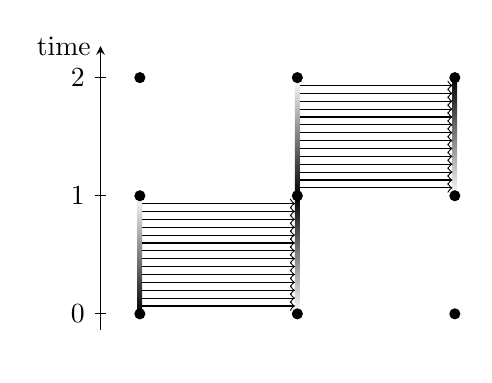
\begin{tikzpicture}
      \tikzstyle{node}=[circle, fill, inner sep =.05cm]
      \tikzstyle{arc} = [draw, thick, -stealth]
      \path[draw, -stealth] (-.5cm,-.2cm) --node[at end,auto]{time} (-.5cm,3.4cm);
      \path[draw,] (-.575cm,0cm) -- (-.425cm,0cm) node[at start, anchor=east] {0};
      \path[draw,] (-.575cm,1.5cm) -- (-.425cm,1.5cm) node[at start, anchor=east] {1};
      \path[draw,] (-.575cm,3cm) -- (-.425cm,3cm) node[at start, anchor=east] {2};
      \foreach \pos/\name in {{(0cm,-0.4cm)/}, {(2cm,-0.4cm)/}, {(4cm,-0.4cm)/}} {\node (\name) at \pos {\name};}
      \shade[top color=white,bottom color=white,middle color=white] (0,0) rectangle (2,1.5);
      \shade[top color=black,bottom color=white,middle color=gray] (1.97,0) rectangle (2.03,1.5);
      \shade[top color=white,bottom color=white,middle color=white] (2,1.5) rectangle (4,3);
      \shade[top color=black,bottom color=white,middle color=gray] (3.97,1.5) rectangle (4.03,3);
      \shade[top color=white,bottom color=black,middle color=gray] (1.97,1.5) rectangle (2.03,3);
      \shade[top color=white,bottom color=black,middle color=gray] (-.03,0) rectangle (0.03,1.5);
      \foreach \pos/\name in {{(0cm,0cm)/1}, {(0cm,1.5cm)/2}, {(0cm,3cm)/3}, {(2cm,0cm)/4}, {(2cm,1.5cm)/5}, {(2cm,3cm)/6},
      {(4cm,0cm)/7}, {(4cm,1.5cm)/8}, {(4cm,3cm)/9}} {\node[node] (\name) at \pos {};}
      \foreach \x in {1,...,14}{\draw[black,->] (0.03cm,0.1*\x cm) -- (1.97cm,0.1*\x cm) node[at start, anchor=east] {};}
      \foreach \x in {16,...,29}{\draw[black,->] (2.03cm,0.1*\x cm) -- (3.97cm,0.1*\x cm) node[at start, anchor=east] {};}
     \end{tikzpicture}}
    \subfigure[\label{fig:ex1Back}Residual network.]{
    \begin{tikzpicture}
        \tikzstyle{node}=[circle, draw]
      \tikzstyle{arc} = [draw, thick, -stealth]
      \foreach \pos/\name in {{(0cm,0cm)/}, {(2cm,0cm)/}, {(4cm,0cm)/}} {
        \node[node] (\name) at \pos {\name};      }
      \foreach \tail / \head / \cap / \cost in {{///}, {///}} {
        \path[arc] (\tail) to [bend left=45]  (\head) node[above,text centered,midway]{\cap}; \path[arc] (\tail) to [bend left=45]  (\head) node[below,text centered,midway]{\cost};}
      \foreach \tail / \head / \cap / \cost in {{///}, {///}} {
        \path[arc] (\head) to [bend left=45]  (\tail) node[above,text centered,midway]{\cost}; \path[arc] (\head) to [bend left=45]  (\tail) node[below,text centered,midway]{\cap};}
          \end{tikzpicture}}
       \hspace{1cm}
    \subfigure[\label{fig:ex1ResExpa}Residual network in time expanded network. The direction of horizontal arrows shows the direction of arcs with positive residual capacity. The up/down-direction of vertical arrows shows the positive upper/lower residual capacity at the nodes.]{
    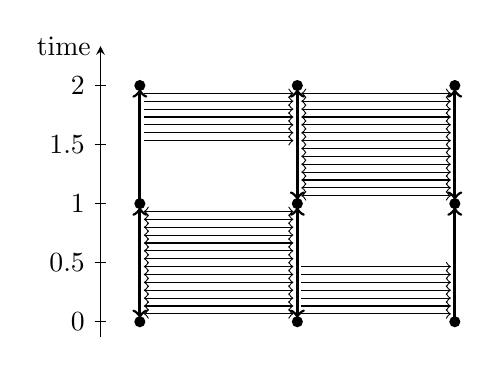
\begin{tikzpicture}
      \tikzstyle{node}=[circle, fill, inner sep =.05cm]
      \tikzstyle{arc} = [draw, thick, -stealth]
      \path[draw, -stealth] (-.5cm,-.2cm) --node[at end,auto]{time} (-.5cm,3.5cm);
      \path[draw,] (-.575cm,0cm) -- (-.425cm,0cm) node[at start, anchor=east] {0};
      \path[draw,] (-.575cm,1.5cm) -- (-.425cm,1.5cm) node[at start, anchor=east] {1};
      \path[draw,] (-.575cm,3cm) -- (-.425cm,3cm) node[at start, anchor=east] {2};
      \path[draw,] (-.575cm,0.75cm) -- (-.425cm,0.75cm) node[at start, anchor=east] {0.5};
      \path[draw,] (-.575cm,2.25cm) -- (-.425cm,2.25cm) node[at start, anchor=east] {1.5};
      \foreach \pos/\name in {{(0cm,-0.4cm)/}, {(2cm,-0.4cm)/}, {(4cm,-0.4cm)/}} {\node (\name) at \pos {\name};}
      \foreach \pos/\name in {{(0cm,0cm)/1}, {(0cm,1.5cm)/2}, {(0cm,3cm)/3}, {(2cm,0cm)/4}, {(2cm,1.5cm)/5}, {(2cm,3cm)/6},
      {(4cm,0cm)/7}, {(4cm,1.5cm)/8}, {(4cm,3cm)/9}} {\node[node] (\name) at \pos {};}
      \foreach \x in {1,...,14}{\draw[black,<->] (0.05cm,0.1*\x cm) -- (1.95cm,0.1*\x cm);}
      \foreach \x in {1,...,7}{\draw[black,->] (2.05cm,0.1*\x cm) -- (3.95cm,0.1*\x cm);}
      \foreach \x in {23,...,29}{\draw[black,->] (0.05cm,0.1*\x cm) -- (1.95cm,0.1*\x cm);}
      \foreach \x in {16,...,29}{\draw[black,<->] (2.05cm,0.1*\x cm) -- (3.95cm,0.1*\x cm);}
      \path[draw,,line width=1pt,<->] (0,0.05) -- (0,1.45);
      \path[draw,,line width=1pt,->] (0,1.55) -- (0,2.95);
      \path[draw,,line width=1pt,<->] (2,0.05) -- (2,1.45);
      \path[draw,,line width=1pt,<->] (2,1.55) -- (2,2.95);
      \path[draw,,line width=1pt,->] (4,0.05) -- (4,1.45);
      \path[draw,,line width=1pt,<->] (4,1.55) -- (4,2.95);
     \end{tikzpicture}}
\caption{\label{fig:AugPath}Network for Example~\ref{ex:AugPath}.}
\end{figure}

We consider the network shown in Fig.~\ref{fig:ex1Orig}.
The transit costs and transit capacities are as follows:

The storage capacities are given as

The transit times and storage costs are assumed to be zero. The problem is to send an initial storage of one
unit from node 1 to node 3 within the time interval~. One possible solution  is obtained as follows. We send flow into arc  with rate  within the interval . The flow arriving at node  is stored there till time . So there will be one unit of flow at node  at time . We send this amount of flow into arc  with rate  within the interval . Fig.~\ref{fig:ex1Expa} shows the flow~ in the corresponding time-expanded network.
Formally,  is given by

with corresponding storage


We are now interested in identifying the augmenting paths and augmenting cycles. Fig.~\ref{fig:ex1Back} depicts the network with backward arcs and Fig.~\ref{fig:ex1ResExpa} depicts the paths and cycles with positive residual capacities in the corresponding time-expanded network. However, there are more augmenting paths and cycles in addition to those shown in Fig.~\ref{fig:ex1ResExpa}, whose residual capacities are zero. Some of them are given below

with costs

and

We observe that the equality  does not hold for some path or cycle .

As mentioned already above, an augmenting path (or cycle) must satisfy the conditions \eqref{it:AugPath1}-\eqref{it:AugPath4}. But the other direction may not hold, that is,
a path satisfying these conditions is not necessarily an augmenting path in general. The following paths and cycles show this fact:


\end{example}


Now let  be an arc-subpath of . We have observed that there exists an (inclusion-wise) maximal closed interval , say, containing  so that the path , given by \eqref{eq:P(alpha)}, is an augmenting path for every . We define a cost function  with respect to  as

where . We recall that  and  for . For the case that , we define , where  is given by \eqref{eq:aug-cost'}. The function  is lower semi-continuous at any point  and such a function attains its local minimum on a closed interval. This fact shows that Theorem~\ref{thm:CDSP-existence} and \ref{thm:CDSP-analytic} hold.


We next proceed to show that the results in Section~\ref{sec:OptCond} are still valid. We consider a feasible flow  and suppose that  is an augmenting cycle. We have defined the cost of  in two different ways:  in terms of the cost of arc-subpaths of  and  as the sum of the costs of the arcs at the times they appear around the cycle . Further, we have observed that these two values are not equal in general. However, we have the following result taht provides another characterization of augmenting cycles with negative cost.

\begin{lemma}
\label{lem:neg-aug-cycle}
Let  be a piecewise analytic flow. The network  contains a negative augmenting cycle if and only if there is a cycle  with  and \mbox{}.
\end{lemma}
\begin{proof}
Suppose first that  is a cycle with  and . Clearly  is an augmenting cycle since . So we need to show that . Recall that  where sum is taken over all maximal arc-subpaths  of~ and  is computed by \eqref{eq:cost}. For each maximal arc-subpath  of , we define  where the index  varies from~ to . The fact that  implies that there exists some  so that  is an augmenting cycle for each . Due to the definition of  and  and the fact that cost functions are right-continuous, we can conclude . Therefore,  which gives the result in one direction.

To prove the other direction, suppose that  is a negative augmenting cycle. Let  be a maximal arc-subpath of . Then we know that there is some  such that  is also an augmenting cycle for each  in  or . We assume without loss of generality that  is an augmenting cycle for each  in . Then for some , we have . Here  denotes the arc path  with starting time . More precisely, we have  where  and  for .
Further,  can be chosen in such a way that . Now we consider the cycle  and repeat the above procedure for all remaining maximal arc-subpaths of . Let  be the resulting cycle. It is easy to see that for sufficiently small , we get  and .
\qed
\end{proof}

This lemma  implies that all results in Section~\ref{sec:OptCond} remain valid even if the cost functions have some discontinuities.

\end{document}
